\chapter{Phương pháp}
\label{chap:method}

Chương này trình bày cách xây dựng mẫu nghiên cứu, quá trình phát triển kiến trúc và hoạt động của mô hình cuối. Ký hiệu $M$, $R$ và $C$ lần lượt chỉ embedding MRI, radiomics và clinical tại một visit. Các khối fusion được dùng chung giữa ba visits; mô hình thời gian sau đó tổng hợp chuỗi thành một điểm nguy cơ ở cấp bệnh nhân. Kết quả dùng để đánh giá các quyết định thiết kế được trình bày riêng ở Chương~\ref{chap:results}.

\section{Thiết kế nghiên cứu và xây dựng dữ liệu}
\label{sec:study-design}

\subsection{Tiêu chí chọn mẫu và ba visits}
Dữ liệu được lấy từ Alzheimer's Disease Neuroimaging Initiative (ADNI), một nghiên cứu dọc đa trung tâm về suy giảm nhận thức và AD \cite{weiner2015impact,jack2008adnimri}. Pipeline liên kết định danh bệnh nhân PTID--RID và chọn baseline MCI sớm nhất có ngày hợp lệ, mã diagnosis bằng 2 và visit code \texttt{bl} trong ADNI1, ADNIGO hoặc ADNI2. Với bệnh nhân $i$, đặt $b_i$ là ngày baseline và $L_i=b_i+18$ tháng lịch là \emph{mốc xét điều kiện cohort}.

Bệnh nhân bị loại nếu có diagnosis AD trong DXSUM, MMSE $<24$ hoặc CDR-global $\geq1$ tại hoặc trước $L_i$. Sau $L_i$, cần ít nhất một đánh giá MMSE/CDR hợp lệ để xác định event hoặc censoring. Đây là một cohort được xây dựng hồi cứu và điều kiện hóa trên việc chưa tiến triển qua cửa sổ 18 tháng; nó không đại diện cho mọi bệnh nhân MCI tại baseline.

MRI được chọn trong khoảng $[b_i,L_i]$. Các scan gần nhau được nhóm thành timepoint theo cửa sổ hai tháng tính từ scan đầu nhóm. Trong mỗi nhóm, scan primary được ưu tiên trước repeat, rồi đến processing rank và image ID. Nếu có hơn ba timepoints, giữ scan đầu, scan cuối và scan trung gian gần trung điểm thời gian nhất. Metadata QC chính thức không liên kết được với image ID của danh sách MRI hiện có, nên lựa chọn sử dụng processing fallback đã ghi trong manifest. Quy trình tạo ra ba ngày MRI tăng nghiêm ngặt $s_{i1}<s_{i2}<s_{i3}\leq L_i$.

\begin{figure}[tbp]
\centering
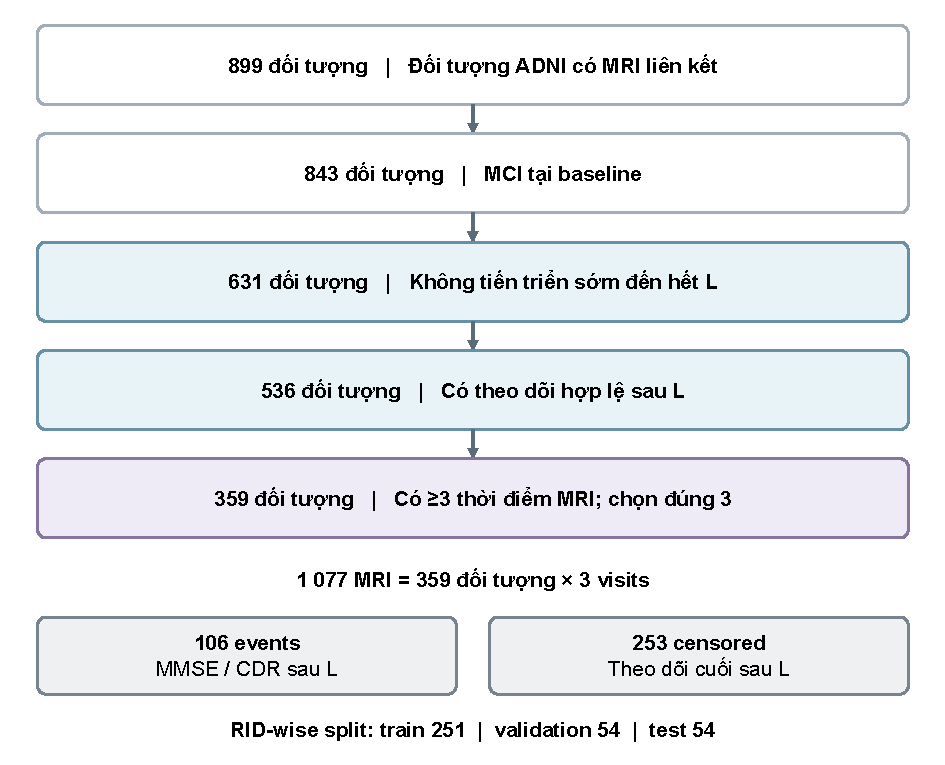
\includegraphics[width=\textwidth]{image/cohort-construction.pdf}
\caption[Quy trình xây dựng cohort dọc]{Quy trình xây dựng cohort từ metadata ADNI đến mẫu ba visits và phép chia theo RID. Số người ở các bước là số liệu của cohort đã đóng băng; MRI, radiomics và clinical được liên kết theo cùng định danh visit trước modeling.}
\label{fig:cohort}
\end{figure}

Hình~\ref{fig:cohort} tóm tắt quá trình lọc từ 899 người có MRI và liên kết định danh thành công xuống 359 người với đúng ba MRI mỗi người, tương ứng 1\,077 MRI. Cohort gồm 106 events và 253 trường hợp censored; phân bố baseline phase là ADNI1: 78, ADNIGO: 80 và ADNI2: 201. Không điều chỉnh tiêu chí để ép cỡ mẫu giống nghiên cứu tham chiếu.

\subsection{Event, censoring và mốc tính thời gian}
Sau $L_i$, event được xác định ở ngày đầu tiên có MMSE hợp lệ $<24$ hoặc CDR-global hợp lệ $\geq1$. Nếu không có event theo quy tắc này, censoring diễn ra ở ngày MMSE/CDR hợp lệ cuối cùng. Những giá trị không hợp lệ hoặc sentinel không tạo event. Endpoint này là \emph{proxy tiến triển dựa trên ngưỡng thang điểm}; nó không đòi hỏi một diagnosis AD sau $L_i$ và không xác nhận AD bằng biomarker.

Ngày tham chiếu dự báo của mô hình là $p_i=s_{i3}$, tức MRI được chọn cuối cùng. Nếu $o_i$ là ngày event hoặc censoring, nhãn survival là
\begin{equation}
 t_i=\frac{o_i-p_i}{365.25},\qquad
 \delta_i=\begin{cases}1,&\text{có event},\\0,&\text{censored}.\end{cases}
 \label{eq:survival-target}
\end{equation}
Do $p_i\leq L_i$, ngày MRI cuối và mốc xét điều kiện cohort không nhất thiết trùng nhau. Nhãn dùng thời gian từ $p_i$, trong khi mẫu đã được chọn với điều kiện không tiến triển đến $L_i$. Khoảng $[p_i,L_i]$ và điều kiện sống sót qua cửa sổ này phải được giữ rõ khi diễn giải, thay vì coi protocol hiện tại là một đánh giá tiến cứu cho mọi bệnh nhân ngay tại $p_i$.

\subsection{Phân chia và bảo vệ quá trình học}
Split cố định theo RID gồm 251 training, 54 validation và 54 test; mọi MRI của một người thuộc cùng một split. Số events tương ứng là 74, 16 và 16. Khóa liên kết xuyên modality là $(\mathrm{RID},\mathrm{visit\_index},\mathrm{image\_id},\mathrm{split})$, với kiểm tra duy nhất và bằng nhau về keyset. Imputer, scaler, loại đặc trưng hằng và PCA đều chỉ fit trên training. Diagnosis, event, ngày outcome và survival time không thuộc tập predictor.

Clinical được ghép với MRI bằng quy tắc frozen: cùng RID, đánh giá hợp lệ gần nhất trong cửa sổ \emph{$\pm90$ ngày}; hòa khoảng cách ưu tiên ngày sớm hơn rồi ID nhỏ hơn. Audit nguồn ghi nhận 294 offset MMSE/CDR dương trên các visits, với khoảng offset từ $-90$ đến $+90$ ngày. Đây là số offset đánh giá được ghép, không phải số bệnh nhân. Vì vậy, bảo vệ train-only và split không đồng nghĩa mọi predictor đã sẵn có vào ngày MRI cuối. Việc dùng clinical sau MRI trong cửa sổ ghép là giới hạn về tính khả dụng khi dự báo tiến cứu, cần kiểm tra bằng protocol chỉ dùng thông tin có trước ngày dự báo ở nghiên cứu tiếp theo.

\section{Tiền xử lý và biểu diễn từng modality}
\label{sec:preprocessing}

\begin{figure}[tbp]
\centering
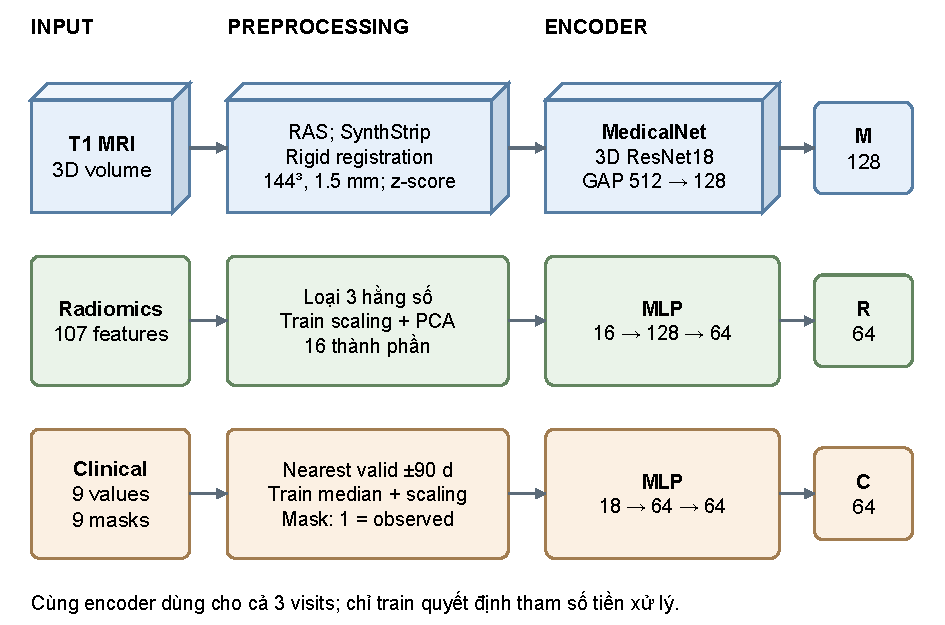
\includegraphics[width=\textwidth]{image/modality-preprocessing.pdf}
\caption[Ba nhánh xử lý modality]{Ba nhánh xử lý tại một visit. MRI tạo embedding $M$ 128 chiều; 16 thành phần radiomics PCA tạo $R$ 64 chiều; 9 giá trị clinical và 9 observedness masks tạo $C$ 64 chiều. Các biến đổi thống kê được fit trên training và giữ cố định khi áp dụng cho validation.}
\label{fig:modalities}
\end{figure}

\subsection{MRI và shared encoder}
Pipeline MRI T1 chuẩn hóa orientation RAS, dùng SynthStrip để tách não \cite{hoopes2022synthstrip}, đăng ký rigid 6-DOF các visits sau về visit đầu, rồi đăng ký rigid visit đầu về MNI152NLin2009cAsym. Ba MRI của cùng người nằm trên lưới chung $144\times144\times144$, spacing 1.5~mm isotropic. Ảnh được z-score trong brain mask riêng của volume; voxel ngoài mask bằng không. Nội suy ảnh là linear và nội suy mask là nearest-neighbor. Pipeline này không bổ sung N4, affine scaling hay nonlinear registration.

Encoder là MONAI ResNet-18 3D dùng chung trọng số giữa visits \cite{he2016deep,cardoso2022monai}. Backbone chứa BatchNorm và ReLU \cite{ioffe2015batchnorm,nair2010rectified}; sau global pooling, vector 512 chiều qua Linear $512\to128$, GELU, Dropout 0.20 và LayerNorm để tạo $M$ \cite{hendrycks2016gelu,srivastava2014dropout,ba2016layernorm}. Trong kiến trúc cuối, backbone được khởi tạo bằng MedicalNet/Med3D \cite{chen2019med3d}, nạp chặt trọng số và BatchNorm buffers của backbone, loại task head pretrained và fine-tune toàn bộ từ epoch đầu. Các mô hình MRI random và pretrained thuộc giai đoạn đối chứng, không phải hai encoder đồng thời trong pipeline cuối.

\subsection{Radiomics}
PyRadiomics trích 107 đặc trưng whole-brain từ MRI đã xử lý và mask, gồm shape, first-order, GLCM, GLDM, GLRLM, GLSZM và NGTDM \cite{vangriethuysen2017computational}. Protocol deep dùng binCount 64. Ba đặc trưng hằng trên training được loại bỏ, còn 104; scaling và PCA giữ ít nhất 99\% phương sai chỉ fit trên training \cite{jolliffe2016pca}. Dữ liệu model-ready có 16 thành phần PCA mỗi visit. Đây là chiều \emph{đầu vào} radiomics; embedding $R$ có 64 chiều sau MLP $16\to128\to64$, GELU, Dropout 0.20 và LayerNorm cuối nhánh.

\subsection{Clinical và observedness masks}
Chín predictor gồm MMSE-total, CDR-global, CDR-sum-of-boxes và sáu miền CDR: memory, orientation, judgment, community affairs, home/hobbies và personal care \cite{folstein1975mmse,morris1993cdr}. Giá trị thiếu được điền bằng median training của visit tương ứng, với median training tổng thể làm fallback, sau đó chuẩn hóa bằng mean và độ lệch chuẩn training. Chín masks riêng dùng $1$ cho giá trị quan sát được, $0$ cho giá trị thiếu. Ghép giá trị và masks tạo 18 đầu vào cho MLP $18\to64\to64$, GELU, Dropout 0.10 và LayerNorm, sinh $C\in\mathbb R^{64}$. Mask giúp phân biệt quan sát thật với giá trị điền; nó không loại bỏ giới hạn của cửa sổ ghép ngày đã nêu ở Mục~\ref{sec:study-design}.

\subsection{Thư viện và triển khai}
Các mô hình neural được triển khai bằng Python và PyTorch cho tensor, automatic differentiation, tối ưu và huấn luyện trên GPU \cite{paszke2019pytorch}. MONAI cung cấp backbone ResNet 3D cho ảnh y tế \cite{cardoso2022monai}. NumPy xử lý mảng số \cite{harris2020numpy}; pandas phục vụ đọc, ghép và kiểm tra các bảng manifest theo bệnh nhân--visit \cite{mckinney2010pandas}. NiBabel đọc volume NIfTI và thông tin affine trong các loader MRI.

Tiền xử lý dữ liệu bảng dùng scikit-learn cho scaling và PCA \cite{pedregosa2011sklearn}; PyRadiomics trích các descriptor đã nêu ở trên \cite{vangriethuysen2017computational}. Baseline Cox elastic-net, Random Survival Forest và đánh giá dữ liệu kiểm duyệt được xây dựng với scikit-survival \cite{polsterl2020sksurv}. Các script kiểm tra tiền xử lý ảnh có sử dụng Matplotlib để trực quan hóa kết quả kiểm tra \cite{hunter2007matplotlib}.

Prototype Cox ban đầu có backend TorchSurv tùy chọn \cite{monod2024torchsurv}. Các phase pairwise được đối chiếu trong khóa luận có implementation Cox/Breslow riêng, với risk set minibatch và cách xử lý ties được mô tả ở Mục~\ref{sec:training-method}. Việc trích dẫn thư viện xác định hạ tầng phương pháp; thông số của các mô hình và kết quả thực nghiệm vẫn được xác định từ artifact của từng phase.

\section{Quá trình phát triển kiến trúc}
\label{sec:architecture-evolution}
Kiến trúc được phát triển theo từng câu hỏi nghiên cứu, không bắt đầu với CP hay topology RC-Free hoàn chỉnh. MRI Only khảo sát biểu diễn không gian từ MRI cuối; Longitudinal MRI thêm T-LSTM và attention để xử lý chuỗi. Multimodal Concatenation tiếp theo kiểm tra thông tin bổ sung từ radiomics và clinical bằng phép nối đơn giản. Dynamic Pairwise Fusion đưa vào tương tác tường minh giữa từng cặp modality và định tuyến residual. Variant MedicalNet giữ cơ chế fusion nhưng thay khởi tạo backbone, sau đó trở thành reference cho thí nghiệm CP.

\begin{figure}[tbp]
\centering
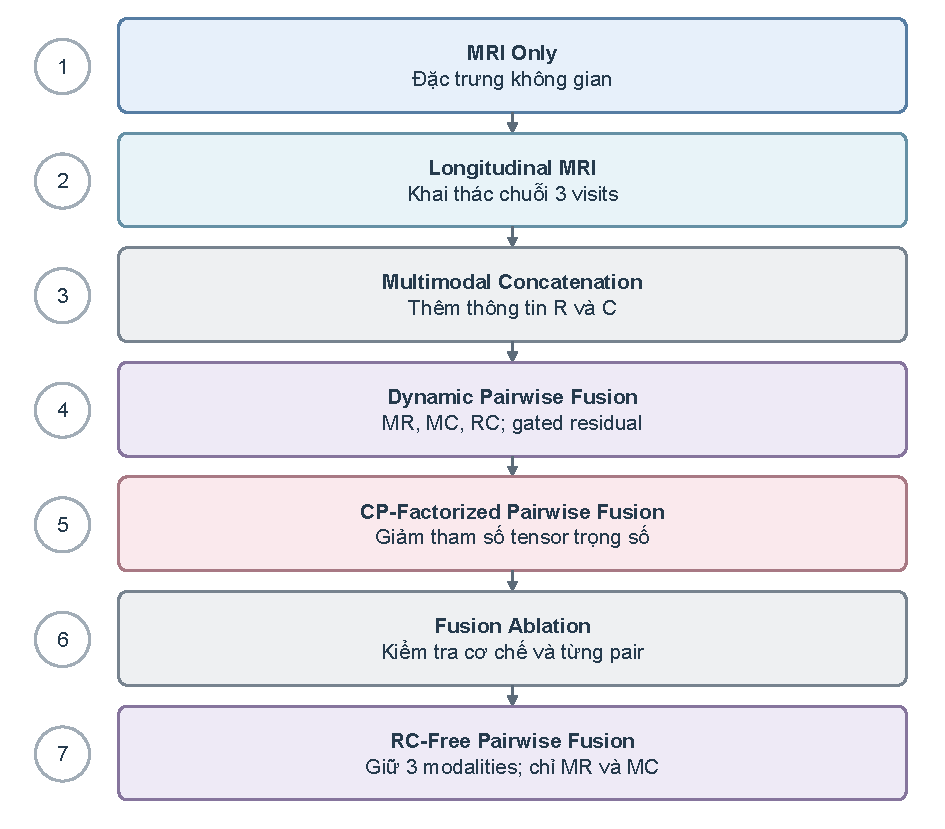
\includegraphics[width=\textwidth]{image/architecture-evolution.pdf}
\caption[Tiến hóa của framework]{Tiến hóa của framework theo các câu hỏi thực nghiệm. CP thay cách tham số hóa interaction core sau khi full outer-product đã được nghiên cứu; topology RC-Free hình thành sau fusion ablation và được kiểm tra tiếp bằng validation nhiều seed.}
\label{fig:evolution}
\end{figure}

Full outer-product tạo tương tác giàu nhưng cần lớp tuyến tính lớn. CP được áp dụng ở bước sau để giảm chi phí của lớp này trong khi giữ các khối còn lại. Fusion ablation tiếp tục kiểm tra gate, scale, identity residual và từng pair. Kết quả validation dẫn tới RC-Free Pairwise Fusion, chỉ giữ MR và MC. Hình~\ref{fig:evolution} là chronology thiết kế; các so sánh và mức độ chắc chắn của bằng chứng được trình bày ở Chương~\ref{chap:results}. Chuỗi milestone ban đầu có khác biệt về protocol batching, nên không được diễn giải toàn bộ thành các đối chứng chỉ thay duy nhất một thành phần.

\section{Multimodal Concatenation baseline}
Tại visit $t$, baseline nối ba embedding:
\begin{equation}
 F_t=\operatorname{Readout}(M_t\concat R_t\concat C_t),\qquad
 M_t\concat R_t\concat C_t\in\mathbb R^{256},\quad F_t\in\mathbb R^{128}.
\end{equation}
Readout gồm Linear $256\to128$, GELU, Dropout 0.20 và LayerNorm. Chuỗi ba $F_t$ đi qua temporal stack và Cox head. Baseline giữ thông tin của cả ba modality nhưng không có bilinear pair block hoặc route riêng, nên tạo mốc so sánh cho câu hỏi về cơ chế interaction.

\section{Dynamic Pairwise Fusion}
Trước khi tạo interaction, các phép chiếu tuyến tính không bias đưa embedding xuống
\begin{equation}
 \widetilde M\in\mathbb R^{32},\qquad
 \widetilde R\in\mathbb R^{32},\qquad
 \widetilde C\in\mathbb R^{16}.
\end{equation}
Những bottleneck này giảm chiều input nhưng full reference vẫn tạo outer-product tường minh. Với pair input $x\in\mathbb R^{d_x}$, $y\in\mathbb R^{d_y}$, đặt $v=\operatorname{vec}(xy^\top)$. MR dùng $1024\to128\to64$, MC dùng $512\to128\to64$, RC dùng $512\to64\to32$. Giữa hai Linear của pair có GELU và Dropout 0.10; cuối pair có LayerNorm.

\begin{figure}[tbp]
\centering
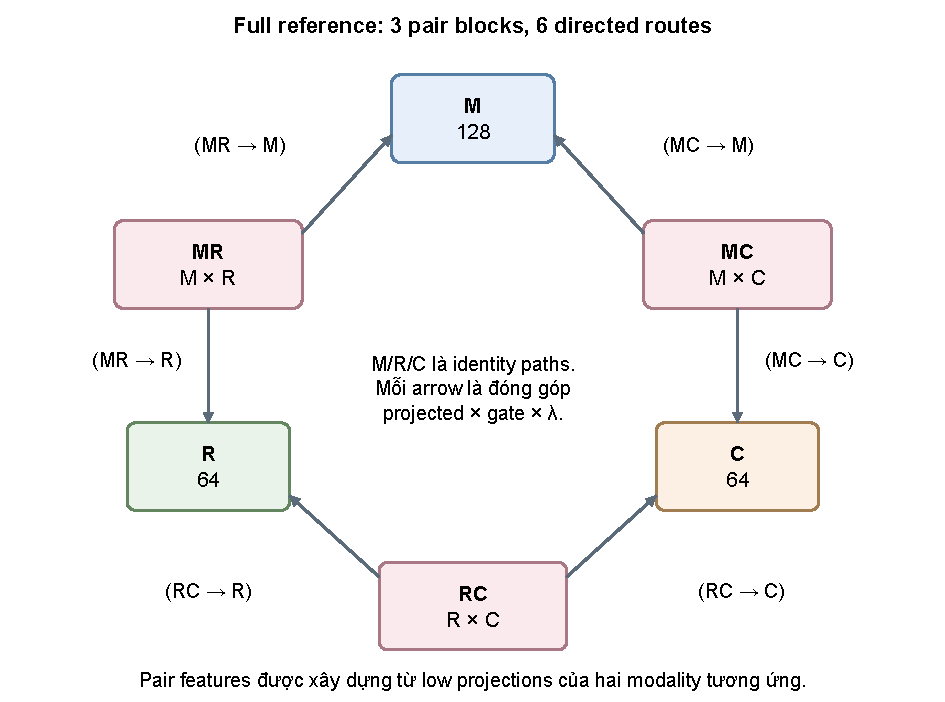
\includegraphics[width=\textwidth]{image/full-pairwise-graph.pdf}
\caption[Full pairwise graph và sáu routes]{Full pairwise graph với ba interaction MR, MC, RC và sáu directed routes về các modality thành viên. Mỗi pair chỉ được tạo một lần tại cùng patient--visit; hai hướng có adapter và gate riêng. Đây là kiến trúc reference trước khi loại RC.}
\label{fig:full-pairwise}
\end{figure}

Mỗi pair feature $E_k$ được đưa về hai modality đích bằng các adapter Linear và LayerNorm độc lập. MR và MC có feature 64 chiều, RC có feature 32 chiều. Sáu output adapter cùng chiều với modality đích: $(\mathrm{MR}\to M)$ và $(\mathrm{MC}\to M)$ là 128; $(\mathrm{MR}\to R)$, $(\mathrm{RC}\to R)$, $(\mathrm{MC}\to C)$ và $(\mathrm{RC}\to C)$ là 64. Interaction chỉ diễn ra trong một visit của một bệnh nhân, không nhân chéo người hoặc thời điểm. Hình~\ref{fig:full-pairwise} tách rõ ba pair blocks và sáu routes thay vì xem các cạnh ngược là sáu pair khác nhau.

\section{CP-factorized pairwise interaction}
\label{sec:cp-method}
Với full bilinear first layer, hidden output thứ $s$ là
\begin{equation}
 h_s=\sum_{i=1}^{d_x}\sum_{j=1}^{d_y}\mathcal W_{sij}x_i y_j+b_s,
 \qquad \mathcal W\in\mathbb R^{d_h\times d_x\times d_y}.
\end{equation}
CP tham số hóa \emph{tensor trọng số của ánh xạ bilinear}, theo dạng low-rank \cite{kolda2009tensor,liu2018lowrank}:
\begin{equation}
 \mathcal W_{sij}\approx\sum_{q=1}^{Q}O_{sq}A_{iq}B_{jq}.
 \label{eq:cp-weight}
\end{equation}
Trong mô hình này $A\in\mathbb R^{d_x\times Q}$, $B\in\mathbb R^{d_y\times Q}$ và $O\in\mathbb R^{d_h\times Q}$ được học cùng mạng. Không có bước phân rã dữ liệu bệnh nhân bằng CP. Forward tương ứng là
\begin{align}
 u&=A^\top x,\qquad v=B^\top y,\qquad q=u\odot v,\\
 h&=Oq+b,\qquad E_{xy}=\operatorname{PostMLP}_{xy}(h).
 \label{eq:cpblock}
\end{align}
$A$ và $B$ không bias; bias $b$ của first layer được giữ trong $Oq+b$. Post-MLP vẫn là GELU, Dropout 0.10, Linear $d_h\to d_o$ và LayerNorm. Vì vậy, controlled CP comparison chỉ thay first interaction transformation, giữ output shape, post-MLP, encoders, routes, gate, scale và temporal stack.

\begin{figure}[tbp]
\centering
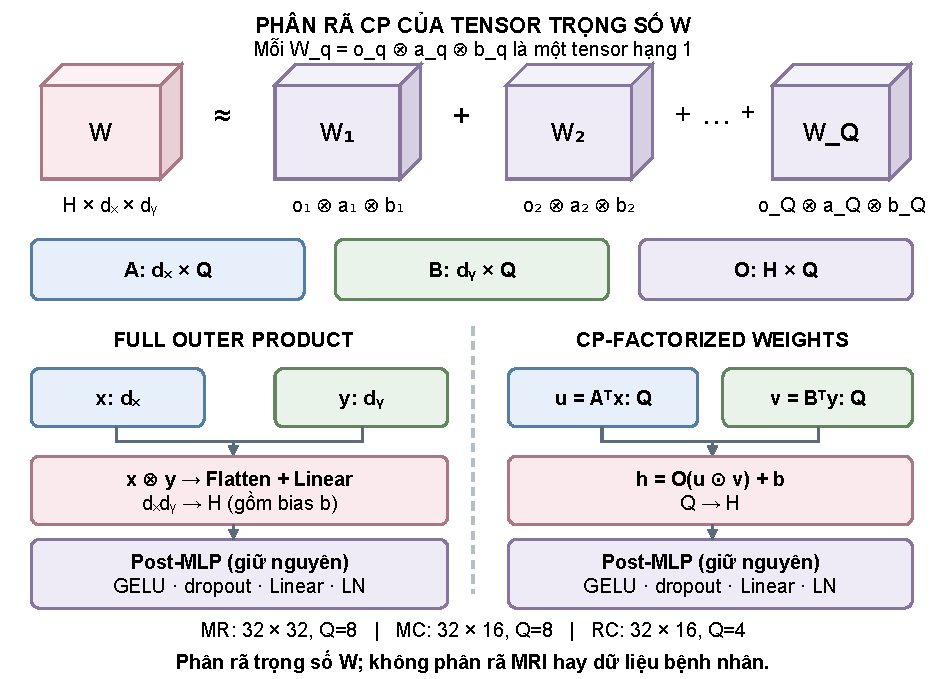
\includegraphics[width=\textwidth]{image/outer-vs-cp.pdf}
\caption[Full outer-product và CP-factorized bilinear]{Full outer-product và CP-factorized first bilinear layer. CP tính hai phép chiếu rank $Q$, tích Hadamard và phép chiếu output mà không tạo activation $d_xd_y$. Post-MLP sau first layer được giữ nguyên trong controlled comparison.}
\label{fig:cp-block}
\end{figure}

\begin{table}[H]
\centering
\caption{Cấu hình CP của full reference và kiến trúc cuối.}
\label{tab:cpconfig}
\begin{tabular}{lccccc}
\toprule
Pair & $(d_x,d_y)$ & Rank $Q$ & Hidden $d_h$ & Output $d_o$ & RC-Free \\
\midrule
MR & $(32,32)$ & 8 & 128 & 64 & Giữ \\
MC & $(32,16)$ & 8 & 128 & 64 & Giữ \\
RC & $(32,16)$ & 4 & 64 & 32 & Loại \\
\bottomrule
\end{tabular}
\end{table}

Bảng~\ref{tab:cpconfig} ghi rank thực sự được dùng; không có kết quả khảo sát rank rộng được tuyên bố trong khóa luận. First layer full có $d_hd_xd_y+d_h$ tham số; CP có $Q(d_x+d_y+d_h)+d_h$. Lợi ích trực tiếp nằm ở interaction core, trong khi backbone MRI vẫn chiếm phần lớn tổng tham số. Không suy ra mức tăng tốc toàn pipeline chỉ từ công thức tham số.

\section{Dynamic gated residual routing}
\label{sec:gated-routing}
Lấy cảm hứng từ gated residual modulation của Ryumina và cộng sự \cite{ryumina2026residual} và explicit residual scaling của Liu và cộng sự \cite{liu2026motion}, khóa luận xây dựng cập nhật residual riêng cho từng route. Hai công trình này cung cấp ý tưởng điều tiết và scaling; công thức dưới đây là thiết kế của project, không phải công thức nguyên dạng của các paper.

Với pair $k$ và modality đích $d$, ký hiệu $U_d$ là embedding modality gốc và
\begin{equation}
 \widehat E_{k\to d}=\LN_{k\to d}(W_{k\to d}E_k+b_{k\to d})
\end{equation}
là feature đã chiếu về chiều đích. Gate dùng cả trạng thái modality và feature route:
\begin{equation}
 g_{k\to d}=\sigma\!\left(
 w_{k\to d}^{\top}\operatorname{GELU}\!\left[
 V_{k\to d}\bigl(\LN_d^{\rm gate}(U_d)\concat\widehat E_{k\to d}\bigr)
 +a_{k\to d}\right]+c_{k\to d}\right).
 \label{eq:dynamic-gate}
\end{equation}
Gate MLP có hidden 32 và output một scalar trong $(0,1)$ cho mỗi patient--visit; scalar được broadcast trên các feature channels. Các routes dùng sigmoid độc lập, không cạnh tranh bằng softmax. Gate weights được khởi tạo Xavier và biases bằng không.

\begin{figure}[tbp]
\centering
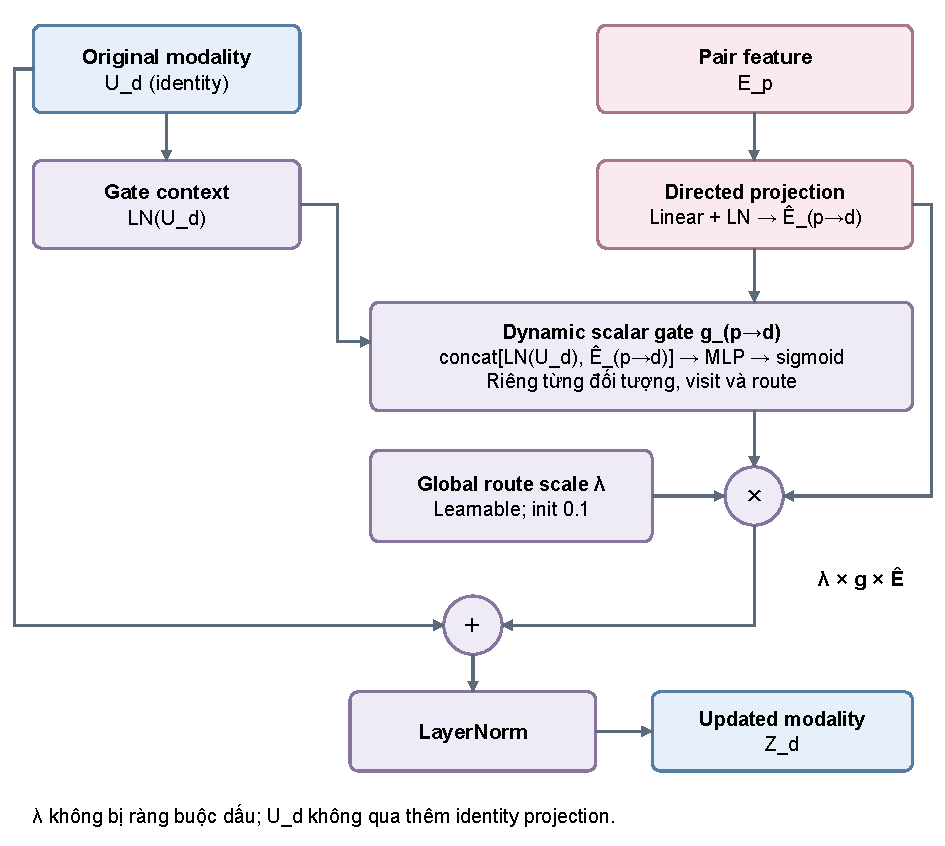
\includegraphics[width=\textwidth]{image/gated-residual-route.pdf}
\caption[Giải phẫu một gated residual route]{Giải phẫu một route: pair feature qua directed projection, nhân dynamic gate theo patient--visit và global route scale, cộng vào đường identity của modality đích rồi LayerNorm. Gate nhận modality gốc đã chuẩn hóa và directed pair feature; đường identity giữ nguyên embedding gốc trước phép cộng.}
\label{fig:route}
\end{figure}

Scale $\lambda_{k\to d}$ là scalar học được riêng cho route nhưng dùng chung giữa bệnh nhân và visits. Implementation hiện có khởi tạo $\lambda=0.1$ và \emph{không ràng buộc dấu}: đây là tham số trực tiếp, không qua softplus. Vì vậy gate biểu diễn mức điều tiết phụ thuộc input, còn $\lambda$ biểu diễn scale và dấu toàn cục của route; không đồng nhất chúng thành attention weight.

Cập nhật tổng quát của modality là
\begin{equation}
 Z_d=\LN_d^{\rm out}\left(
 U_d+\sum_{k\in\mathcal P(d)}\lambda_{k\to d}\,g_{k\to d}\,\widehat E_{k\to d}
 \right).
 \label{eq:ours-residual}
\end{equation}
$\mathcal P(d)$ là các pair còn hoạt động đi vào $d$. Đường identity dùng trực tiếp $U_d$, không thêm một phép chiếu identity học được. LayerNorm ở adapter, ở input gate và sau tổng residual là ba phép chuẩn hóa khác nhau \cite{ba2016layernorm}. Contribution thực tế phụ thuộc đồng thời $\lambda$, gate và norm feature; riêng gate hoặc scale không chứng minh ý nghĩa sinh học hay quan hệ nhân quả.

\section{RC-Free Pairwise Fusion}
\label{sec:rcfree-method}
Kiến trúc cuối cho nghiên cứu validation là RC-Free CP-Factorized Pairwise Fusion, gọi ngắn là RC-Free Pairwise Fusion. Quyết định bỏ RC được nghiên cứu sau full CP ablation rồi kiểm tra tiếp bằng nhiều seed; nó không phải giả định được áp đặt từ đầu. RC-Free loại \emph{direct radiomics--clinical pair}, đồng thời vẫn giữ cả ba unimodal branches. MRI trở thành điểm nối của hai interaction MR và MC.

Đặt $D_{k\to d}=\lambda_{k\to d}g_{k\to d}\widehat E_{k\to d}$, các output là
\begin{align}
 M_{\rm out}&=\LN_M^{\rm out}(M+D_{(\mathrm{MR}\to M)}+D_{(\mathrm{MC}\to M)}),\\
 R_{\rm out}&=\LN_R^{\rm out}(R+D_{(\mathrm{MR}\to R)}),\\
 C_{\rm out}&=\LN_C^{\rm out}(C+D_{(\mathrm{MC}\to C)}).
 \label{eq:rcfree-residual}
\end{align}

\begin{figure}[tbp]
\centering
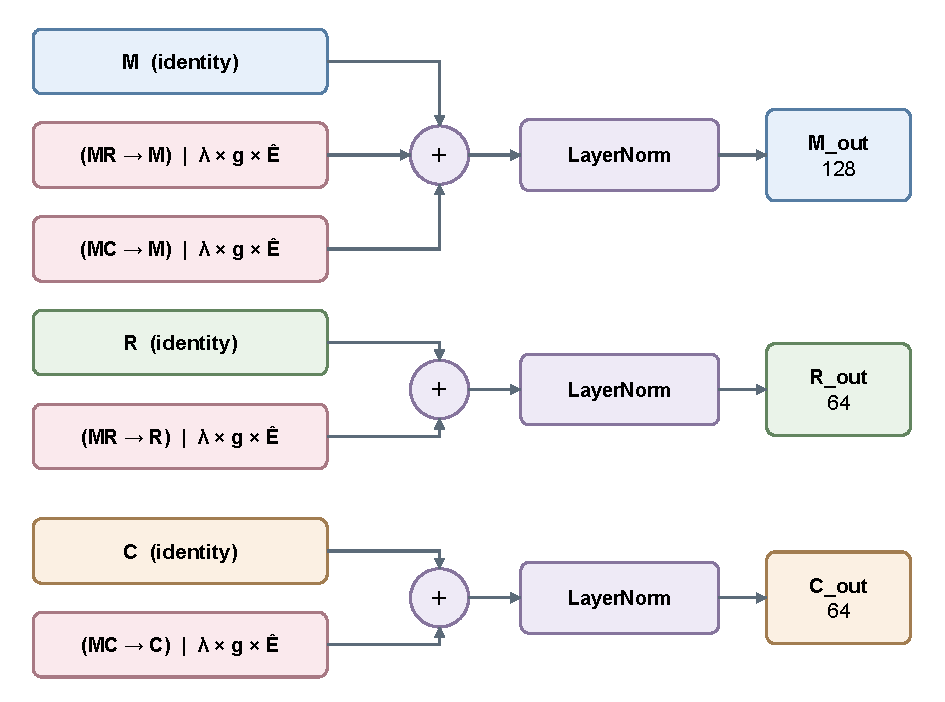
\includegraphics[width=\textwidth]{image/rc-free-routing.pdf}
\caption[Residual routing của RC-Free Pairwise Fusion]{Residual routing của RC-Free Pairwise Fusion theo ba hàng modality đích. MRI nhận MR và MC, radiomics nhận MR, clinical nhận MC. Mỗi hàng giữ đường identity, cộng contribution rồi LayerNorm; $(\mathrm{RC}\to R)$ và $(\mathrm{RC}\to C)$ không hoạt động.}
\label{fig:rcfree-routing}
\end{figure}

Hai CP blocks MR/MC dùng ranks 8/8; bốn directed adapters, bốn dynamic gates và bốn learnable scales còn hoạt động. Output vẫn là 128/64/64, nên downstream readout và temporal model không đổi. Biến thể RC-Free Fixed-$\lambda$ chỉ cố định bốn scales bằng 0.1 để khảo sát sensitivity, không thay thế kiến trúc chính. Loại một interaction không đồng nghĩa kết luận hai modality vô ích hoặc độc lập về mặt y học.

\section{Tổng quan pipeline cuối}
\label{sec:final-pipeline}
Hình~\ref{fig:overall} liên kết toàn bộ các bước. Tại mỗi visit, ba branches tạo $M_t,R_t,C_t$; hai CP pair blocks tạo MR và MC; gated residual routing tạo $M_{{\rm out},t},R_{{\rm out},t},C_{{\rm out},t}$. Phép nối giữ thứ tự MRI--radiomics--clinical, sinh 256 chiều và readout xuống $F_t\in\mathbb R^{128}$. Chuỗi $(F_1,F_2,F_3)$ cùng các khoảng cách ngày MRI đi vào T-LSTM, attention và Cox head.

\begin{figure}[tbp]
\centering
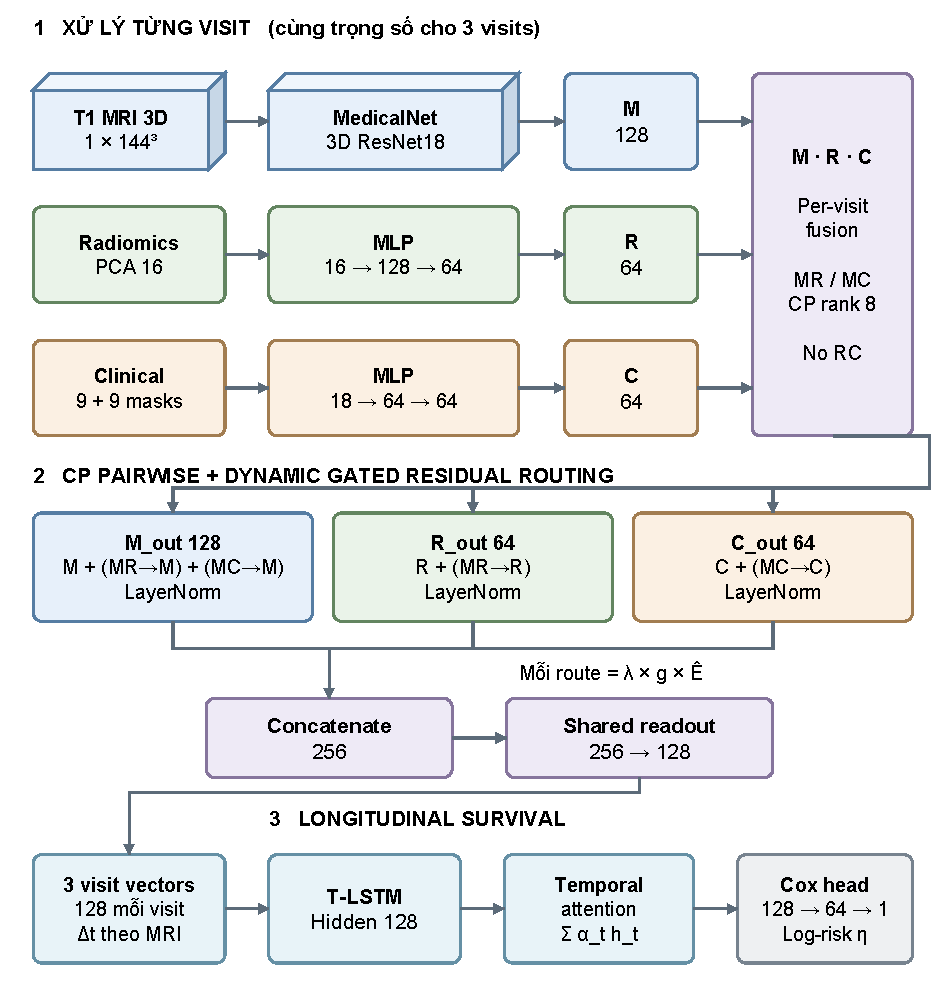
\includegraphics[width=\textwidth]{image/final-pipeline.pdf}
\caption[Kiến trúc tổng thể của framework cuối]{Kiến trúc tổng thể của Longitudinal Learning with Tensor Fusion. Phần trên xử lý một visit bằng ba encoders, CP interactions MR/MC và gated residual routing; phần dưới tổng hợp ba visit embeddings bằng T-LSTM và temporal attention, sau đó xuất raw Cox log-risk. Không có direct RC interaction trong pipeline cuối.}
\label{fig:overall}
\end{figure}

\begin{table}[H]
\centering
\caption{Kích thước tensor chính trong kiến trúc cuối, với batch size $B$.}
\label{tab:pipeline-shapes}
\begin{tabularx}{\textwidth}{Yl}
\toprule
Tensor & Shape \\
\midrule
MRI sequence & $[B,3,1,144,144,144]$ \\
Radiomics PCA & $[B,3,16]$ \\
Clinical values / observedness masks & $[B,3,9]$ / $[B,3,9]$ \\
$M_{\rm out},R_{\rm out},C_{\rm out}$ & $[B,3,128]$, $[B,3,64]$, $[B,3,64]$ \\
Readout / T-LSTM hidden sequence & $[B,3,128]$ \\
Temporal attention weights & $[B,3]$ \\
Subject embedding / raw log-risk & $[B,128]$ / $[B]$ \\
\bottomrule
\end{tabularx}
\end{table}

\section{Mô hình thời gian và temporal attention}
\label{sec:temporal-method}
T-LSTM xử lý khoảng cách visit không đều qua sự suy giảm short-term memory \cite{baytas2017patient,aghajanian2025longitudinal}. Khoảng thời gian đầu bằng không; các khoảng còn lại là $\Delta t_t=(s_t-s_{t-1})/365.25$, đo bằng năm. Không dùng số thứ tự visit thay cho khoảng ngày và không thêm learned time embedding.

Từ memory trước đó $c_{t-1}$, cell phân tách và điều chỉnh:
\begin{align}
 c_{t-1}^{S}&=\tanh(W_Sc_{t-1}+b_S),\qquad
 c_{t-1}^{L}=c_{t-1}-c_{t-1}^{S},\\
 \gamma_t&=\frac{1}{\log(e+\Delta t_t)},\qquad
 c_{t-1}^{*}=c_{t-1}^{L}+\gamma_t c_{t-1}^{S}.
 \label{eq:tlstm-memory}
\end{align}
Input, forget, output gates và candidate được tính từ $F_t$ và $h_{t-1}$ bằng các phép chiếu tuyến tính; cell cập nhật
\begin{equation}
 c_t=f_t\odot c_{t-1}^{*}+i_t\odot\widetilde c_t,
 \qquad h_t=o_t\odot\tanh(c_t).
\end{equation}
Mô hình dùng một layer unidirectional, hidden 128. Thời gian tác động vào decay của short-term memory; khi visit mask không hợp lệ, cell giữ trạng thái trước. Cohort hiện có đủ ba visits, nhưng cơ chế mask được giữ trong implementation.

\begin{figure}[tbp]
\centering
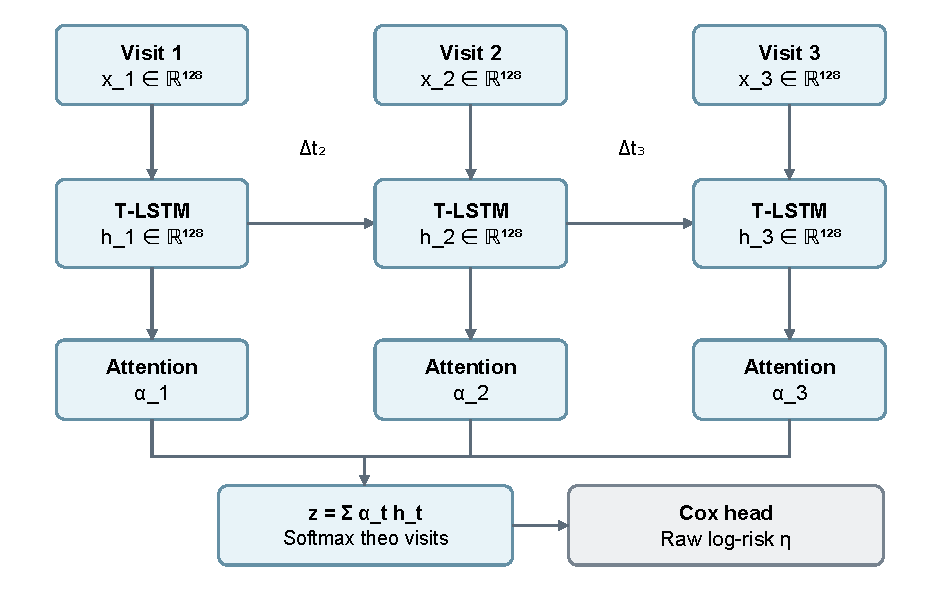
\includegraphics[width=\textwidth]{image/temporal-model.pdf}
\caption[T-LSTM và temporal attention]{Ba visit embeddings và khoảng cách MRI đi qua T-LSTM. Mỗi hidden state được chấm điểm bởi additive attention; tổng có trọng số tạo subject representation cho Cox head. Visit mask điều khiển temporal aggregation, khác với masks cho từng giá trị clinical.}
\label{fig:temporal}
\end{figure}

Masked additive attention lấy cảm hứng từ cơ chế chấm điểm học được \cite{bahdanau2015attention}:
\begin{equation}
 e_t=v_a^\top\tanh(W_a h_t+b_a),\qquad
 \alpha_t=\frac{\exp(e_t)}{\sum_{j\in\mathcal V}\exp(e_j)},\qquad
 z=\sum_{t\in\mathcal V}\alpha_t h_t.
 \label{eq:temporal-attention}
\end{equation}
$\mathcal V$ là tập visits hợp lệ. Attention projection dùng $128\to64\to1$, và $z\in\mathbb R^{128}$. Temporal weights phản ánh cách tổng hợp chuỗi của mạng, không phải mức quan trọng lâm sàng đã được xác nhận của từng visit.

\FloatBarrier
\section{Cox objective, huấn luyện và lựa chọn mô hình}
\label{sec:training-method}
Survival head dùng Linear $128\to64$, GELU, Dropout 0.30 và Linear $64\to1$ để sinh raw log-risk $\eta_i$. Không đặt sigmoid hoặc softmax cuối head. Với giả định proportional hazards \cite{cox1972regression},
\begin{equation}
 h(\tau\mid z_i)=h_0(\tau)\exp(\eta_i).
\end{equation}
Điểm nguy cơ lớn hơn tương ứng nguy cơ event sớm hơn; nó không trực tiếp là xác suất tiến triển ở một horizon cụ thể.

Gọi $\tau_k$ là các event times khác nhau, $\mathcal D_k$ là nhóm events tại $\tau_k$, $d_k=|\mathcal D_k|$ và $\mathcal R_k=\{j:t_j\geq\tau_k\}$. Negative partial log-likelihood với Breslow ties \cite{breslow1974covariance}, trung bình trên số events $N_e$, là
\begin{equation}
 \mathcal L_{\rm Cox}=-\frac{1}{N_e}\sum_k
 \left[\sum_{i\in\mathcal D_k}\eta_i
 -d_k\log\!\left(\sum_{j\in\mathcal R_k}\exp(\eta_j)\right)\right].
 \label{eq:cox-method}
\end{equation}
Trong training thực tế, $\mathcal R_k$ chỉ gồm bệnh nhân trong \emph{physical minibatch}, nên đây là xấp xỉ risk set toàn training cohort. Gradient accumulation không ghép các risk sets thành full-cohort likelihood. Validation loss được tính trên toàn bộ 54 người. Cox arithmetic dùng FP32 và log-sum-exp để giữ ổn định số học.

Protocol chính dùng AdamW \cite{loshchilov2019adamw} với learning rate $10^{-4}$, weight decay $10^{-4}$, betas $(0.9,0.999)$. Physical batch gồm 6 người, tích lũy gradient hai bước; sampling có xét event, không replacement hoặc oversampling. Mô hình dùng AMP FP16, clipping norm 1.0 và tối đa 100 epochs. ReduceLROnPlateau theo full-validation Cox loss dùng factor 0.5, patience 5 và learning rate tối thiểu $10^{-6}$. Early stopping theo validation C-index có warm-up 10 epochs, patience 20 và min-delta 0.002. Best checkpoint được lưu theo validation C-index \cite{harrell1996multivariable}; các run giữ checkpoint cuối để audit trajectory.

Ba seeds 20260727, 20260728 và 20260729 thay đổi khởi tạo, sampling và optimization trên cùng split cố định. Architecture selection sử dụng validation, kiểm tra nhiều seed và standardized validation benchmark; không dùng historical test metrics làm tiêu chí lựa chọn. Formal held-out final evaluation chưa được thực hiện trong phase đánh giá cuối. Kết luận về hiệu năng ở Chương~\ref{chap:results} vì vậy là bằng chứng validation trong cohort và protocol đã mô tả.
